
\documentclass[12pt]{article}
\usepackage[utf8]{inputenc}
\usepackage[T1]{fontenc}
\usepackage{amsmath}

\usepackage{amssymb}
\usepackage{amsmath}
%\usepackage{amsthm}
\usepackage{amsopn}
\usepackage{graphicx}
\usepackage{mathrsfs}
\usepackage{empheq}

\usepackage{tikz}
\usetikzlibrary{fit,positioning}
\usetikzlibrary{arrows}

%\usepackage{showkeys}



%\setlength{\arraycolsep}{2pt}
%\setlength{\parskip}{.04in}
%\setlength{\footskip}{30pt}

\let\bb\mathbb       % BlackBoardBold (double letters)

\def\1{\mathbf 1}

  \def\AA{{\bb A}}\def\CC{{\bb C}}\def\DD{{\bb D}}\def\EE{{\bb E}}
  \def\GG{{\bb G}}\def\HH{{\bb H}}\def\KK{{\bb K}}\def\LL{{\bb L}}
  \def\MM{{\bb M}}\def\QQ{{\bb Q}}\def\TT{{\bb T}}\def\YY{{\bb Y}}
  \def\PP{{\bb P}}\def\II{{\bb I}}\def\WW{{\bb W}}\def\XX{{\bb X}}
  \def\VV{{\bb V}}\def\SS{{\bb S}}\def\BB{{\bb B}}\def\NN{{\bb N}}
  \def\RR{{\bb R}}\def\ZZ{{\bb Z}}\def\FF{{\bb F}}\def\DD{{\bb D}}
  \def\OO{{\bb O}}\def\JJ{{\bb J}}\def\UU{{\bb U}}

\def\cH{\mathcal H}
\def\cY{\mathcal Y}
\def\cX{\mathcal X}
\def\cA{\mathcal A}
\def\mC{\mathcal C}
\def\Ex{\mathbf E}

\def\bb{\mathbb}
%end of header
\def\hat{\widehat}
\def\bfX{\mathbf X}
\def\bfB{\mathbf B}
\def\bSigma{\boldsymbol\Sigma}
\def\bOmega{\boldsymbol\Omega}
\def\bmu{\boldsymbol\mu}
\def\bnu{\boldsymbol\nu}
\def\bPi{\boldsymbol\Pi}
\def\bX{\boldsymbol X}
\def\bx{\boldsymbol x}
\def\bbeta{\boldsymbol \beta}
\def\bY{\boldsymbol Y}
\def\bxi{\boldsymbol \xi}
\def\bpi{\boldsymbol \pi}
\def\ci{\perp\!\!\!\perp}
\def\bZ{\boldsymbol Z}


\newcommand{\argmax}{\arg\!\max}

\parskip=3pt
\renewcommand{\baselinestretch}{1.08}

\title{\vspace{-60pt}~\\Double sparsity in high-dimensional Gaussian mixture estimation and clustering\\Subject Overview}
\author{\vspace{-20pt}~\\ Laboratory Supervisor: A.S. Dalalyan\\
PHd Student: M. Sebbar}
\date{\today}

\begin{document}
\maketitle
\tableofcontents
\newpage
\section{Introduction}
The broad goal of this thesis is to tackle a clustering problem in the scope of mixtures model framework. More precisely, we will study the clustering of points drawn from high-dimensional Gaussian mixtures distributions.\\Thus, in the first part of this section we present the Gaussian mixture model and the second part we describe the well know  Expectation-Maximization algorithm (EM). We will also present the limitations of this algorithm in high-dimensional setting.
\subsection{The Gaussian mixture model}

The Gaussian mixture model is an important framework for clustering problems. The components are Gaussian distributions with parameters $(\mu_i,\Sigma_i)$:
\begin{equation}
\varphi_{(\mu_i,\Sigma_i)}(x)=\frac{1}{(2\pi)^{p/2}|\Sigma_i|^{1/2}} \exp(-\frac{1}{2}(x-\mu_i)^T\Sigma_i^{-1}(x-\mu_i))
\end{equation}

The density is given by:
\begin{equation}
p_{\theta}(x)=\sum_{k=1}^K\pi_k\varphi_{(\mu_k,\Sigma_k)}(x)
\end{equation}
with $\theta=\{(\mu_k,\Sigma_k,\pi_k): 1\leq k\leq K; \; \Sigma_k \geq 0;\; \pi_k>0  \;\forall k\; and \;\sum_{k=1}^K\pi_k=1 \}$
\\

This model can be interpreted from a latent variable perspective. Let $Z$ be a multionomial random variable of parameters $\mu(1,\bpi)$, we have:
\begin{equation}
p_{\theta}(x)=\sum_{k=1}^K P_{\theta}(Z^k=1)p_{\theta}(x|Z^k=1)
\end{equation}
Therefore $\pi_k=p_{\theta}(Z^k=1)$ and reflects the probability that $x$ is drawn from the $k^{th}$ mixture component.\\

In the clustering problem, the goal is to assign $X$ to a cluster and therefore estimate the probability of the latent variable $Z$ conditioned on $X$ which we denote $\tau^k(x,\theta)=p_{\theta}(Z^k=1|x)$. From Bayes's rule we have:

\begin{equation}
\label{tau_bayes}
\tau^k(x,\theta)=\frac{p_{\theta}(x|Z^k=1)P_{\theta}(Z^k=1)}{p_{\theta}(x)}
=\frac{\pi_k\varphi_{(\mu_k,\Sigma_k)}(x)}{\sum_{k'=1}^K\pi_{k'}\varphi_{(\mu_{k'},\Sigma_{k'})}(x)}
\end{equation}

The of estimation  $\tau^k(x,\theta)$ rely on computing the parameters $\theta$. An approach to this problem is to estimate the parameter that maximize the likelihood.\\

Let $X_1,\dots,X_N$ with $X_i\in \RR^p$ a set of iid observations drawn from $p_{\theta}$. The related graphical model is:

%%GRAPH of pgm
\begin{figure}[h]
\centering
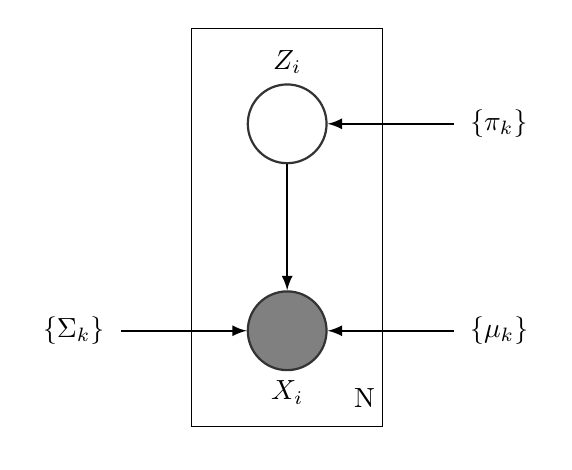
\begin{tikzpicture}
\tikzstyle{main}=[circle, minimum size = 10mm, thick, draw =black!80, node distance = 16mm]

\tikzstyle{connect}=[-latex, thick]
\tikzstyle{box}=[rectangle, draw=black!100]
  \node[main, fill = black!50] (x) [label=below:{$X_i$}] { };
  \node[main] (z) [above=of x,label=above:{$Z_i$}] {};

  \path (z) edge [connect] (x);

  \node[rectangle, inner sep=7mm,draw=black!100, fit= (z) (x)] {};
\node[rectangle, below=of x, inner sep=-10mm, fit= (z) (x),label=below right:N, xshift=7mm,yshift=-9mm] {};

\node[main,draw=none] (a) [right=of x] {$\{\mu_k\}$};
\path (a) edge [connect] (x);
\node[main,draw=none] (b) [left=of x] {$\{\Sigma_k\}$};
\path (b) edge [connect] (x);
\node[main,draw=none] (c) [right=of z] {$\{\pi_k\}$};
\path (c) edge [connect] (z);
\end{tikzpicture}
\end{figure}

The log-likelihood is:

\begin{equation}
l(\theta|x_1,\dots,x_N)=\sum_{i=1}^{N}\log{p_{\theta}(x_i)}=\sum_{i=1}^{N}\log\Big({\sum_{k=1}^K\pi_k\varphi_{(\mu_{k},\Sigma_{k})}(x_i)}\Big)
\end{equation}

In this equation, we have the logarithm of a sum and the maximization of the log-likelihood is a non-linear problem. (This is not a exponential family distribution where the log acts on a simple probability distribution and therefore yields simple expressions).\\
A well known approach for computing the maximum of log-likelihood is the Expectation-Maximization Algorithm \cite{dempster77}.

%%%%%%%%%%%%%%%%%%%

\subsection{The EM Algorithm}

We will infer the values of $\{z_n\}$ conditioned to the data $\{x_n\}$. A natural approach to infer the parameters $\theta$ is to estimate the mean of each class by computing the partial derivative of the log-likelihood with respect to $\mu_k$ and setting to 0. We have:


\begin{equation}
\sum_{i=1}^N\frac{\pi_k\varphi_{(\mu_k,\Sigma_k)}(x_i)}{\sum_{k'=1}^K\pi_{k'}\varphi_{(\mu_{k'},\Sigma_{k'})}(x_i)} \Sigma_k^{-1}(x_i-\mu_k)=\sum_{i=1}^N \tau_i^k \Sigma_k^{-1}(x_i-\mu_k)=0
\end{equation}
Assuming that $\Sigma_k$ is non singular, we have:

\begin{equation}
\label{muk}
\mu_k=\frac{\sum_{n=1}^N\tau_n^k x_n}{\sum_{n=1}^N\tau_n^k}
\end{equation}

Doing a similar computation for $\Sigma_k$, we have:

\begin{equation}
\label{sigmak}
\Sigma_k=\frac{\sum_{n=1}^N \tau_n^k (x_n-\mu_k)(x_n-\mu_k)^T}{\sum_{n=1}^N\tau_n^k}
\end{equation}

Finally, maximizing the log-likelihood with respect to $\pi_k$ with the condition $\sum_{k=1}^K\pi_k=1$ (using Lagrange multiplier), we have:
\begin{equation}
\label{pik}
\pi_k=\frac{\sum_{n=1}^N\tau_n^k}{N}
\end{equation}

However, as seen in \eqref{tau_bayes}, $\tau_n^k$ depends on the parameter estimatation $\hat\theta$ which depends on $\tau_n^k$ as seen in \eqref{muk},\eqref{sigmak} and \eqref{pik}. An idea would be to initialize the parameters and iterate. We calculate the posterior probability and then estimate the parameter $\theta$. This is the idea of the EM algorithm.
\\

\subsubsection{The EM algorithm for Gaussian Mixtures:}
\begin{enumerate}
\item[0.] Initialize parameters $\mu_k^0,\; \Sigma_k^0,\;\pi_k^0$
\item Calculate (Expectation Step):
\begin{equation}
\label{posteriorEM}
\tau_i^k(t+1)=\frac{\pi_k(t) \varphi_{(\mu_k(t),\Sigma_k(t))}(x_i)}{\sum_{k'=1}^K\pi_{k'}(t)\varphi_{(\mu_{k'},\Sigma_{k'})}(x_i)}
\end{equation}
\item Calculate (Maximization Step):\\

We note: $\rho^k_i(t+1)=\frac{\tau_i^k(t+1)}{\sum_{j=1}^N\tau_j^k(t+1)}$, hence:

\begin{align}
\mu_k(t+1)&=\sum_{i=1}^N \rho^k_i(t+1) x_i\\
\Sigma_k(t+1)&=\sum_{i=1}^N \rho^k_i(t+1) (x_i-\mu_k(t+1))(x_i-\mu_k(t+1))^T\\
\pi_k(t+1)&=\frac{\sum_{i=1}^N\tau_i^k(t+1)}{N}
\end{align}


\item Evaluate the log-likelihood and check for convergence as explained in the following section
\end{enumerate}

\subsubsection{An analysis of the EM Algorithm convergence}
\label{sec:emconv}

As defined previously, we denote all observed variables $\bX$ and discrete variables $\bZ$. Our goal is to maximize the likelihood function\cite{Bishop}:

\begin{equation}
l(\theta|\bX)=log (p_{\theta}(\bX))=log\Big(\sum_{\bZ}p_{\theta}(\bX,\bZ) \Big)
\end{equation}
We introduce a distribution $q(\bZ)$ over the latent variables. We have:

\begin{equation}
\label{klem}
l(\theta|\bX)=\mathcal{L}(q,\theta)+KL(q||p_{\theta})
\end{equation}

with:
  \begin{align}
\mathcal{L}(q,\theta)&=\sum_{\bZ}q(\bZ)\log\Big(\frac{p_{\theta}(\bX,\bZ)}{q(\bZ)}\Big)\\
KL(q||p_{\theta})&=-\sum_{\bZ}q(\bZ)\log\Big(\frac{p_{\theta}(\bZ|\bX)}{q(\bZ)}\Big)
  \end{align}

To verify this identity, we will start by decomposing $\mathcal{L}(q,\theta)$:

\begin{align}
\mathcal{L}(q,\theta)&=\sum_{\bZ}q(\bZ)\log\Big(\frac{p_{\theta}(\bX,\bZ)}{q(\bZ)}\Big)=\sum_{\bZ}q(\bZ)\log\Big(\frac{p_{\theta}(\bX)p_{\theta}(\bZ|\bX)}{q(\bZ)}\Big)\\
&=\sum_{\bZ}q(\bZ)\log\Big(\frac{p_{\theta}(\bZ|\bX)}{q(\bZ)}  \Big)  +\sum_{\bZ}q(\bZ)\log p_{\theta}(\bX)\\
&=-KL(q||p_{\theta})+l(\theta|\bX)
\end{align}

$KL(q||p_{\theta})$ is the Kullback-Leibler divergence between $q(\bZ)$ and $p_{\theta}(\bZ|\bX)$. It satisfies $KL(q||p_{\theta})\geq0$. Therefore, $\mathcal{L}(q,\theta)\leq l(\theta|\bX) $. With the decomposition (\ref{klem}) we will prove that EM maximize the log-likelihood.\\

If we observe the E-Step of EM, we hold $\theta^{old}=\{(\mu_k(t),\Sigma_k(t),\pi_k(t))\}$ and optimize the lower bound $\mathcal{L}(q,\theta^{old})$ with respect to $q$. Because $l(\theta^{old}|\bX)$ does not depend on $q(\bZ)$, we need to decrease $KL(q||p_{\theta^{old}})$ which disappear when $q^{new}(\bZ)=p_{\theta^{old}}(\bZ|\bX)$ as seen in (\ref{posteriorEM}). At this Step:

\begin{equation}
  \mathcal{L}(q^{new},\theta^{old})=l(\theta^{old}|\bX)
\end{equation}

In the M-Step, $q^{new}(\bZ)$ is fixed and we optimize $\mathcal{L}(q^{new},\theta)$ with respect to $\theta$. $l(\theta|\bX)$ depends on $\theta$ and will increase, fixing a new likelihood. And by optimizing $\theta$, $q(\bZ)$ is no longer equal to $p_{\theta^{new}}(\bZ|\bX)$ and we have a nonzero Kullback-Leibler divergence. Therefore, $l(\theta|\bX)$ will increase greater than $\mathcal{L}(q^{new},\theta)$\\

If we decompose $\mathcal{L}(q,\theta)$:

\begin{align}
\mathcal{L}(q^{new},\theta)&=\sum_{\bZ}p_{\theta^{old}}(\bZ|\bX)\log\Big(\frac{p_{\theta}(\bX,\bZ)}{p_{\theta^{old}}(\bZ|\bX)}\Big)\\
&=\sum_{\bZ}p_{\theta^{old}}(\bZ|\bX)\log p_{\theta}(\bZ|\bX) - \sum_{\bZ}p_{\theta^{old}}(\bZ|\bX)\log p_{\theta^{old}}(\bZ|\bX)\\
&=\mathcal{Q}(\theta,\theta^{old})+H(q)
\end{align}

$\mathcal{Q}(\theta,\theta^{old})$ is the expectation of the complete log-likelihood and $H(q)$ is the entropy of $q$. Therefore, the M-Step is equivalent to maximize $\mathcal{Q}(\theta,\theta^{old})$ with respect to $\theta$:

\begin{equation}
  \theta^{new}=\argmax_{\theta}(\mathcal{Q}(\theta,\theta^{old}))
\end{equation}

A variant of EM, the Generalized EM (GEM) is based on the idea that it suffices to increase $Q$ and not necessarily find the maximum.(ref)\\

As we saw in this section, each steps increase the log-likelihood and yields to a local maximum. By running EM over different initial parameters, we improve the estimation by choosing the best local maximum found.

\subsubsection{Stopping criterion of EM}
.
\subsubsection{Limitations of the EM Algorithm:}

EM is conceptually easy and each iteration increases $l(\theta)$. However, the complexity at each step of EM algorithm is $O(dn+Kn^2)$ and it requires many iterations. Unfortunately, in our case, the algorithm slows down in the high dimensional setting. We hope to tackle this problem by making sparsity assumptions on the structure of the precision matrix $\Sigma^{-1}$.

%%%%%%%%%%%%%%%%%%%%%%
\section{Draft-A structural analysis on $\bSigma$ approach}

We consider a multivariate Gaussian distribution with mean $\bmu^*$ and covariance $\bSigma^*$ and $Y_1,\dots,Y_N \in \RR^p$ iid drawn from this distribution. We would like to estimate $\bmu^*$ and $\bSigma^*$. We know that $\hat\bmu_n=\bar Y_n$, then wlog we consider $\mu^*=0$, the problem is to estimate $\bSigma^*$. We will study the precision matrix and consider that $\Sigma^{-1}$ is sparse. We note $\Sigma^{-1}=\Omega$, $Y_n$ the $n$-th random variable and $Y_n^i$ the $i$-th component of this vector.\\
If $\Sigma^{-1}_{ij}=0 \Rightarrow Y^i \ci Y^j$ conditionally to $Y^{l\ne\{i,j\}}$. Thus, it makes sense to impose a $L_1$ penalty on $\Sigma^{-1}$ to increase its sparsity.

\subsection{Graphical Lasso}
Let consider a multivariate normal distribution with parameters $\mu^*,\; \Sigma^*$ with density;
\begin{equation}
\mathcal N(x|\mu^*,\Sigma^*)
=\frac{1}{(2\pi)^{d/2}|\Sigma^*|^{1/2}}\exp^{-\frac{1}{2}(x-\mu^*)^T\Sigma^{-1*}(x-\mu^*)}
\end{equation}
We consider $\mu=0$. Given N datapoints $X_1,\dots,X_N$ and $X_i \in \RR^d$, the log-likelihood is given by:
\begin{equation}
\begin{split}
\mathcal{L}(\Sigma)=\log\left(\prod_{n=1}^N\frac{1}{(2\pi)^{d/2}|\Sigma|^{1/2}}\exp^{-\frac{1}{2}(x_n)^T\Sigma^{-1}(x_n)}\right)\\
=-\frac{dN}{2}\log 2\pi - \frac{N}{2}\sum_{n=1}^N\log |\Sigma^*|- \frac{1}{2}\sum_{n=1}^N x_n^T\Sigma^{*,-1}x_n
\end{split}
\end{equation}
Note that $x_n^T\Sigma^{*,-1}x_n=tr(x_n^T\Sigma^{*,-1}x_n)$, and therefore:
\begin{equation}
\sum_{n=1}^N x_n^T\Sigma^{*,-1}x_n=tr\big(\sum_{n=1}^N x_n^T\Sigma^{*,-1}x_n\big)=tr\Big(\big[\sum_{n=1}^N x_n^Tx_n\big]\Sigma^{*,-1}\Big)=tr(S_N\Sigma^*)
\end{equation}
Where $S_N$ is the empirical covariance matrix. We can replace that in the log-likelihood expression:
\begin{equation}
\mathcal{L}(\Sigma)=-\frac{dN}{2}\log 2\pi - \frac{N}{2}\sum_{n=1}^N\log |\Sigma^*|- \frac{1}{2}tr(S_N\Sigma^*)
\end{equation}
Finally:
\begin{equation}
\mathcal{L}(\Sigma)=C+\frac{N}{2}\log|\Sigma^{-1}|-\frac{1}{2} tr(S_n\Sigma^{-1})
\end{equation}

Where C is a constant (dependent on N). Thus, considering the sparsity of the precision matrix $\Omega=\Sigma^{-1}$, we impose a penalization to the maximum likelihood estimator of $\Omega$
\begin{equation}
\hat\Omega\in argmin\big\{ \log|\Omega|-tr(S_N\Omega)-\lambda||\Omega||_1   \big\}
\end{equation}
A reason to use the $L_1$ penalization instead of the ridge is that for an $L_p$ penalization, the problem is convex for $p\geq 1$ and we have parsimonious property for $p\leq 1$.\\
This is a convex optimization problem, however the complexity is $O(p^3)$ (Source, high dim \& var select Buhlmann 2006 ? Wassermann)
\subsection{Column-Wise Lasso}

We consider a gaussian vector $Y\in \RR^d$, $Y \sim \mathcal N(0,\Sigma)$. We can write $Y=(Y^1,Y^{2:d})$. With this decomposition we can write the covariance matrix as following:
\begin{equation}
\Sigma=
 \begin{pmatrix}
\sigma_1^2 & \Sigma_{12}\\
\Sigma_{12}^T & \Sigma_{22}
\end{pmatrix}
\end{equation}
and according to theorem[?]: If $\Sigma_{22}$ is inversible, then:
\begin{equation}
\begin{array}{lcl}
\EE[Y^1|Y^{2:d}]&=&\Sigma_{12}\Sigma_{22}^{-1}Y^{2:d}\\
Var[Y^1|Y^{2:d}]&=&\sigma_1^2-\Sigma_{12}\Sigma_{22}^{-1}\Sigma_{12}^T
\end{array}
\end{equation}
We have the following identity:
\begin{equation}
 \begin{pmatrix}
 \omega_{11}&\Omega_{12}\\
 \Omega_{12}^T&\Omega_{22}
\end{pmatrix}
 \begin{pmatrix}
 \sigma_{1}^2&\Sigma_{12}\\
 \Sigma_{12}^T&\Sigma_{22}
\end{pmatrix}
=
 \begin{pmatrix}
 1&0\\
0&I_{p-1}
\end{pmatrix}
\end{equation}
Which gives the following equations:
\begin{equation}
  \begin{cases}
  \omega_{11}\sigma_1^2+\Omega_{12}\Sigma_{12}^T&=1\quad\,\quad(*) \\
  \omega_{11}\Sigma_{12}+\Omega_{12}\Sigma_{22}&=0\quad\,\quad(**)\\
  \Omega_{12}^T\Sigma_{12}+\Omega_{22}\Sigma_{22}&=I_{p-1}\quad(***)
  \end{cases}
\end{equation}
With (**) we have $-\omega_{11}\Sigma_{12}\Sigma_{22}^{-1}=\Omega_{12}$ and injected to (*) we have:
\begin{equation}
 \begin{cases}
 \EE[Y^1|Y^{2:d}]&=-\frac{1}{\omega_{11}}\Omega_{12}Y^{2:d}\\
  Var[Y^1|Y^{2:d}]&=\frac{1}{\omega_{11}}
  \end{cases}
\end{equation}
Finally, $Y^1-\EE[Y^1|Y^{2:d}]$ is a gaussian vector of $\RR^{d-1}$, centered, independent of $Y^{2:d}$ and of covariance matrix $\sigma_1^2-\Sigma_{12}\Sigma_{22}^{-1}\Sigma_{12}^T$. If we denote  $\xi^1\sim \mathcal N(0,1)$ we have $Y^1-\EE[Y^1|Y^{2:d}]=\frac{1}{ \sqrt{\omega_{11}}}\xi^1$.\\

Therefore, for $Y_1,\dots,Y_n$ iid of law $\mathcal N(0,\Sigma^*)$ we have:

\begin{equation}
\begin{array}{lcl}
  Y_i^1&=&-\frac{1}{\omega_{11}^*}\Omega_{12}Y_i^{2:d}+\frac{1}{\sqrt{\omega_{11}^*}}\xi^1_i\\
  &=&-\sum_{j=2}^{d}\frac{w_{ij}^*}{\omega_{11}^*}Y_i^j+\frac{1}{\sqrt{\omega_{11}^*}}\xi^1_i
\end{array}
\end{equation}

and
\begin{equation}
{\beta_1^*}^TY_i=\frac{1}{\sqrt{\omega_{11}^*}}\xi^1_i
\Rightarrow
{\beta_1^*}^T\bY=\frac{1}{\sqrt{\omega_{11}^*}}\bxi^1
\end{equation}
with
\begin{equation}
\beta_1^*=\frac{1}{\sqrt{\omega_{11}^*}}
  \begin{bmatrix}
  w_{11}^*\\
  w_{12}\\
  \vdots\\
  w_{1d}
  \end{bmatrix}
  \in \RR^d
  \quad \text{and}\quad \bY= \begin{bmatrix}
  verifier\\
  \end{bmatrix}
\end{equation}


\subsection{The Square-Root Lasso}

\section{Comments}
\bibliographystyle{plain}
\bibliography{ref}

\end{document}
